\chapter{Question 4}
\section{Questions}
Calculate $\lim_{x\to-\infty} \frac{3x^3 + x^2 + 42}{3|x|^3 + |x| +1}$ if it
exists. Check your result on an appropriate graph of the function.

\section{Solutions}
\begin{align}
  \lim_{x\to-\infty} \frac{3x^3 + x^2 + 42}{3|x|^3 + |x| +1} &= ...
  \intertext{It will be valuable to see what the dominant terms are as $x$ tends
  to $-\infty$}
    \frac{3x^3 + x^2 + 42}{3|x|^3 + |x| +1} &= ...
  \intertext{From the numerator, the constants 42 and 3 become less and less
  important, and from the denominator the 3 and 1 become less important. At
  sufficiently large values for $x$, the squared and $|x|$ values become
  inconsequential leading to}
    \frac{x^3}{|x|^3} &= ...
  \intertext{As we are looking at negative values for $x$, the numerator will
  always be negative and the denominator will always be positive. Overall the
  fraction will always be negative because:}
    \frac{(\text{negative})^3}{\text{positive}^3} &= \quad \text{negative}
  \intertext{Divided out, these tend towards}
  &= -1
\end{align}
Using Mathematica to plot the function given the Mathematica command\\
\indent \texttt{
Plot[(3x\^{}3 + x\^{}2 + 42)/(3 (Abs[x])\^{}3 + Abs[x] + 1), {x, -500, 0}]} \\
yields a plot that is asymptotic towards $-1$. The plot is in figure
\ref{fig:q4plot} on page \pageref{fig:q4plot}.
\begin{figure}[!h]
  \centering
  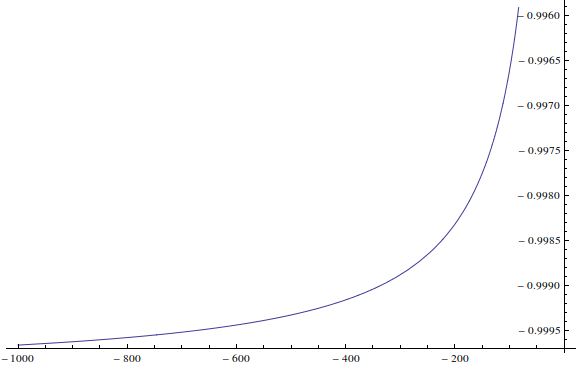
\includegraphics[width=\linewidth]{solutions/q4/q4plot.png}
\caption{Plot of $\frac{3x^3 + x^2 + 42}{3|x|^3 + |x| +1}$ tending to $-1$.}
\label{fig:q4plot}
\end{figure} \\
